
%The lines in this "pre-begin{document}" section can be ordered however you want
%Class of documents; you can also specify the format of your document (a4, a5, ...) and the default size for characters
%\documentclass[12pt, a4paper]{article}
\documentclass{beamer}
\usecolortheme{crane}
%\usecolortheme{wolverine}
%\usecolortheme{orchid}
\usetheme{Copenhagen}  

%The packages you'll be using
%IPA package for IPA symbols
\usepackage{tipa}
%Useful to play with margins (see below)
%\usepackage{geometry}
%\geometry{margin=1in}

%Required for including graphics
\usepackage{graphicx}

%Useful for math mode
\usepackage{amssymb}
\usepackage{amsmath}
\usepackage{amsthm}

%Useful for proofs
%\usepackage{bussproofs}
%\usepackage{proof}

%Required for trees, use "center" and "nocenter" depending on whether you want your trees to be centered
\usepackage[nocenter]{qtree}

%\usepackage{tabularx}

\usepackage{alltt}

\usepackage{hyperref}

%Useful for more complex drawings
\usepackage{tikz}


\usepackage{textcomp}


%Here we start the document we've defined above
\begin{document}
%Automatic heading: our \title and \date are passed to \maketitle below which formats them
\title{\LaTeX Workshop}
\date{\today}
\author{gabriel}
%\author{/g\ae bRi\textipa{E}l/}
\maketitle


\begin{frame}[fragile]
\frametitle{What is \LaTeX}
\begin{itemize}
\item Markup programming language (think of HTML) \pause
\item 2-step document formatting: \LaTeX\ takes in a text file (.tex) and outputs a beautifully formatted document (.pdf or .div or .ps, etc.) \pause
\item Unlike MS Word: ``Everything" is a command, e.g. \verb;{\bf X};, \verb;\maketitle;, \verb;\begin{X};, \verb;\usepackage{X};
\end{itemize}


\end{frame}

\begin{frame}
\frametitle{How to use \LaTeX}
\begin{itemize}
\item You need a \LaTeX distribution that provides you with the actual software plus a lot of commonly used packages:
\begin{itemize}
\item MikTeX or TexLive for Windows
\item MacTeX for OS X
\item TexLive or AucTex for Linux
\end{itemize} \pause
\item You also need some program to write your text with:
\begin{itemize}
\item Tex editors: TexShop, TexMaker, TexWorks
\item Regular text editors work too, but require compiling with terminal as extra step
\end{itemize}
\begin{center}
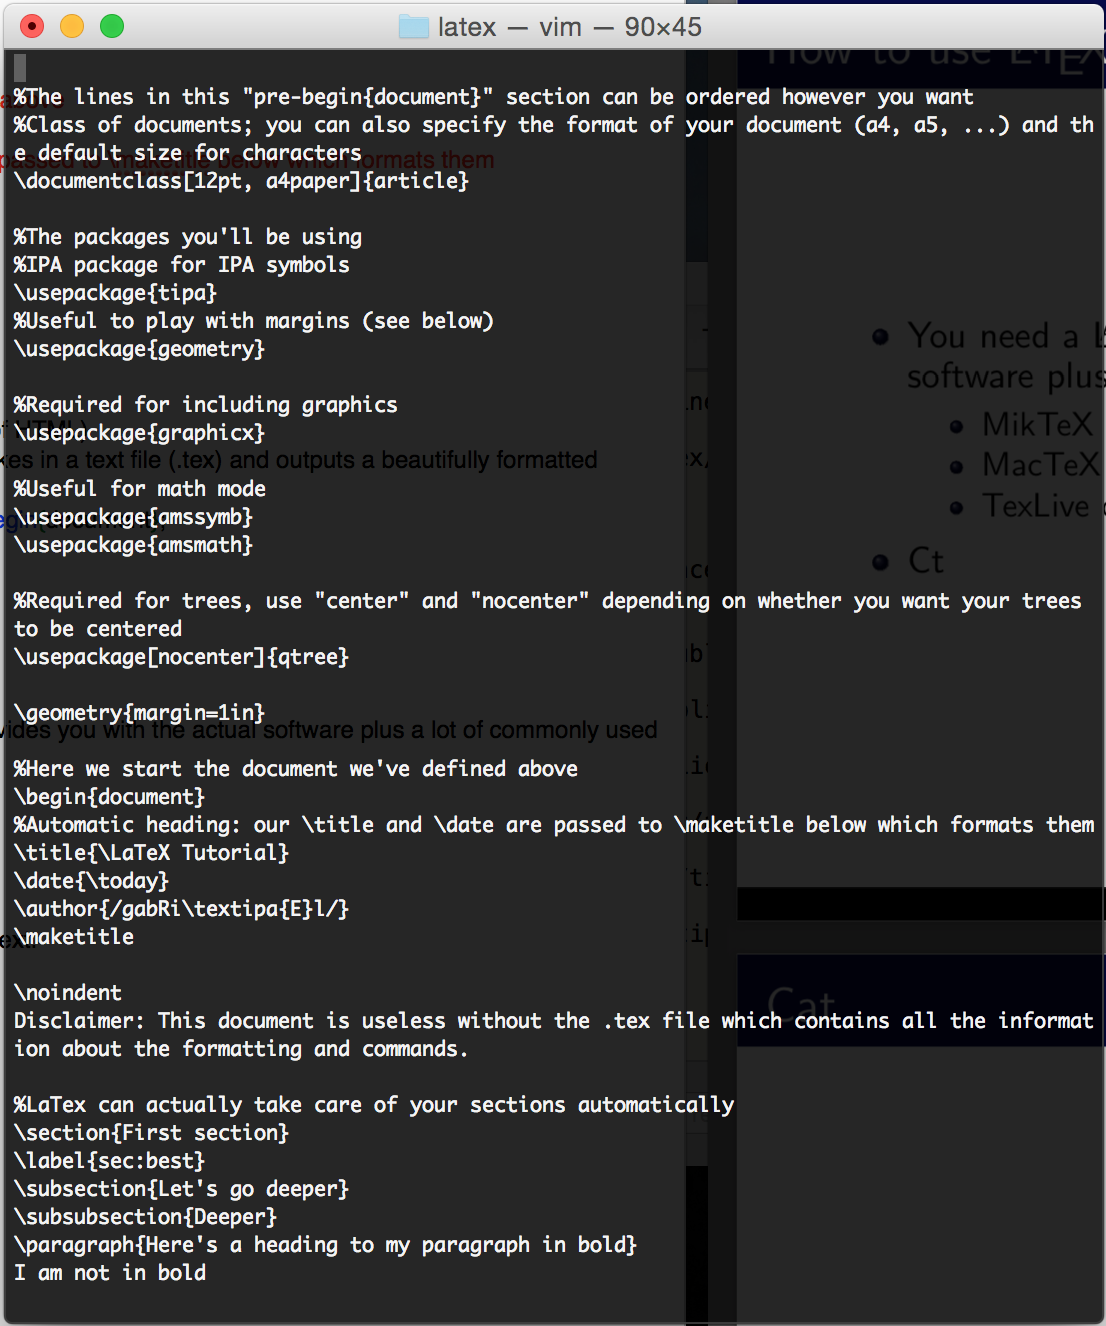
\includegraphics[width=2.5cm]{terminal}
\ \ \ \ 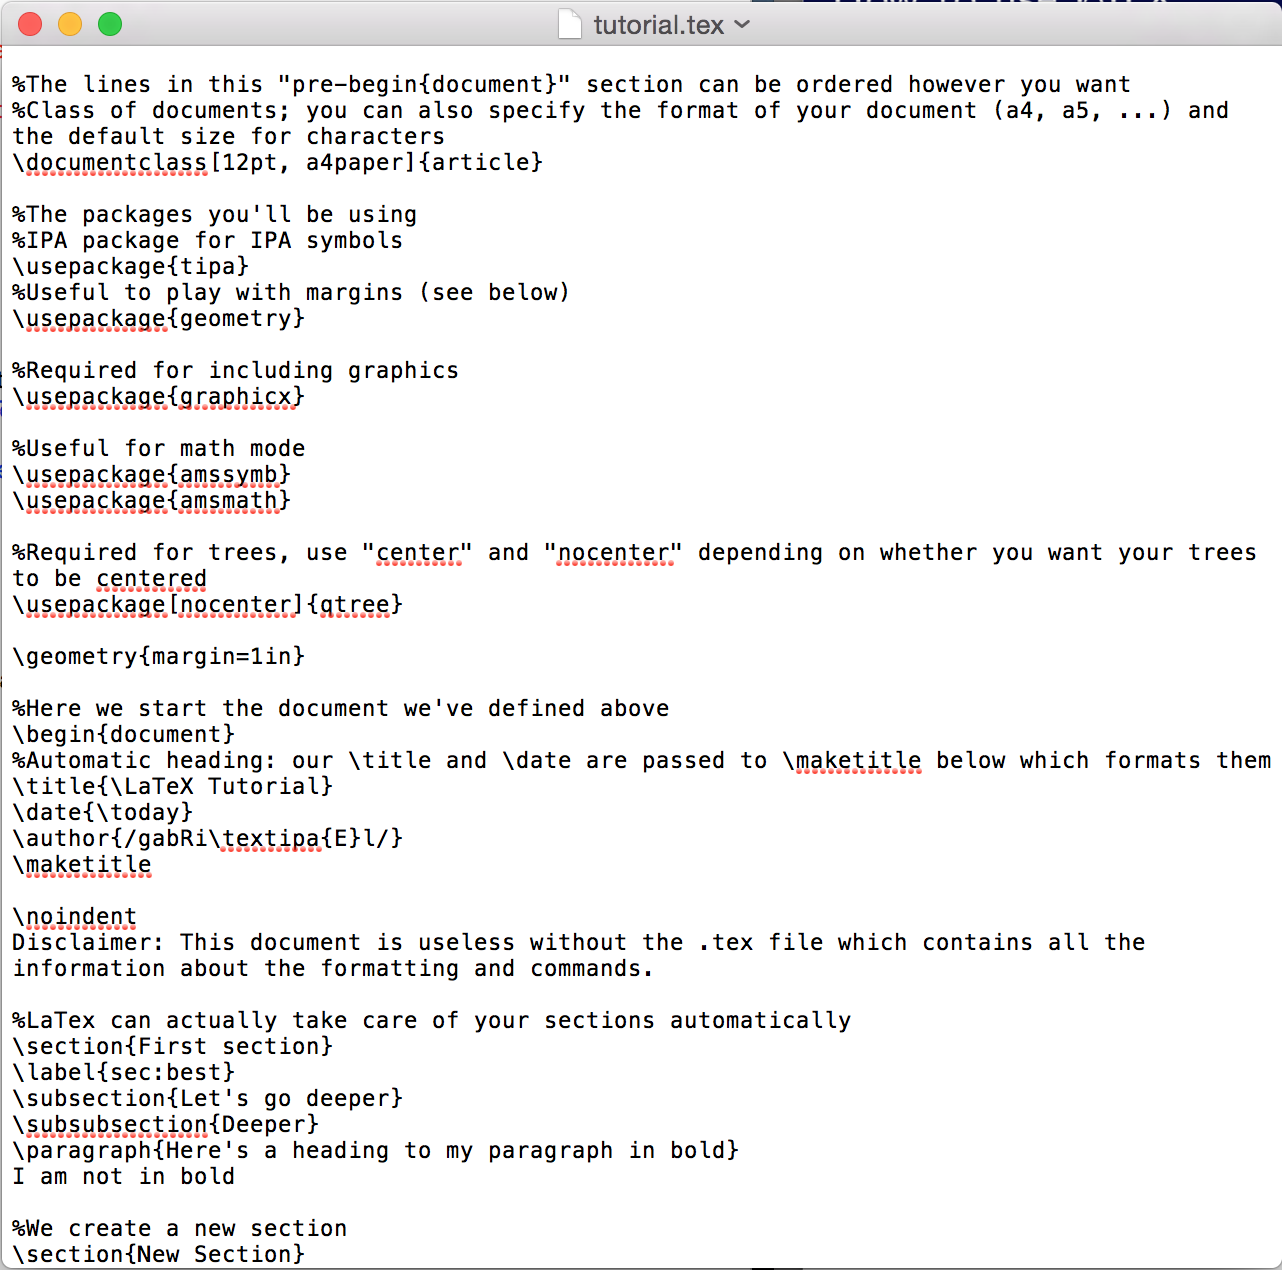
\includegraphics[width=2.5cm]{text_editor}
\ \ \ \ 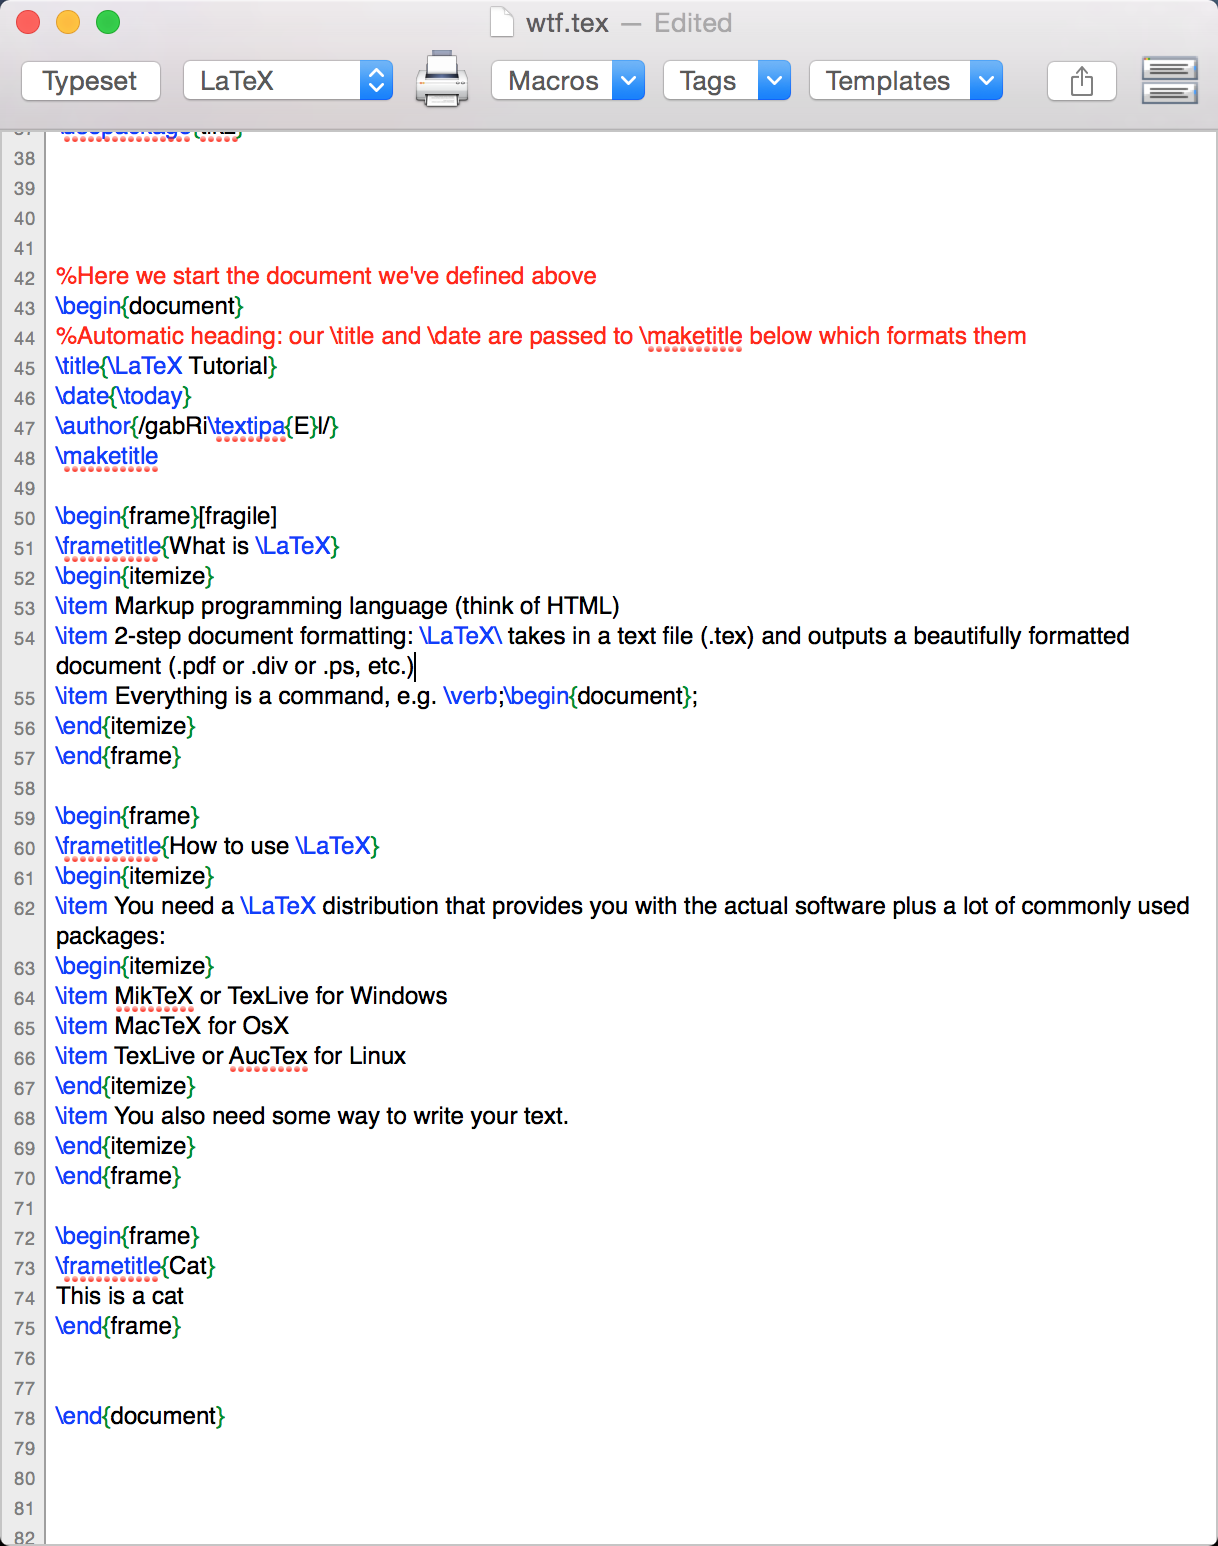
\includegraphics[width=2.5cm]{texshop}
\end{center}
\end{itemize}
\end{frame}

\begin{frame}
\frametitle{Demo}
\begin{center}
{\LARGE DEMO}
\end{center}
\end{frame}

\begin{frame}[fragile]
\frametitle{Basic structure of a document}
\begin{verbatim}
\documentclass{article}

\usepackage{.........}

\begin{document}

 ..........................

\end{document}
\end{verbatim}
\end{frame}



\begin{frame}[fragile]
\frametitle{This document's preamble}
\begin{verbatim}
\documentclass{beamer}
\usecolortheme{crane}
\usetheme{Copenhagen}  
\usepackage{tipa}
\usepackage{hyperref}
\usepackage{graphicx}
\usepackage{amssymb}
\usepackage{amsmath}
\usepackage{amsthm}
\usepackage{alltt}
\usepackage{tikz}
\end{verbatim}
\end{frame}


\begin{frame}[fragile]
\frametitle{(very basic) Slides}
\begin{verbatim}
\documentclass{beamer}
\usecolortheme{crane}
\usetheme{Copenhagen}

\begin{document}  

\begin{frame}
\frametitle{TITLE}
BLA BLI BLO BLU \pause
BLA BLI BLO BLU
 \end{frame}
 
\end{document}

\end{verbatim}

\end{frame}


\begin{frame}[fragile]
\frametitle{Command Formats}

\begin{verbatim}
{\COMMAND1 BLA BLI BLO BLU}  %First command format

\COMMAND2{ BLA BLI BLO BLU} %Second command format

\COMMAND3 %Third command format

\begin{COMMAND4} %Fourth command format
BLA BLI BLO BLU
\end{COMMAND4$}
\end{verbatim}

\end{frame}



%\begin{frame}
%\frametitle{New frame}
%Hello
%\end{frame}



\begin{frame}[fragile]
\frametitle{Basic character styling}
\verb;\begin{enumerate};
\begin{enumerate}
%We can write sentences in italic using \it
\item {\it Italic}\ \ \ \ \ \ \ \ \ \ 
\verb;\item {\it Italic};
%We can write them in bold using \bf
\item {\bf Bold}\ \ \ \ \ \ \ \ \ \ 
\verb;\item {\bf Bold};
%We can also underline text using the \underline command
\item \underline{Underline}\ \ \ \ \ 
\verb;\item {\underline Underline};
%Use \large, \Large, \LARGE, \small for different sizes
\item {\small Small}\ \ \ \ \ \ \ \ \ \ \ 
\verb;\item {\small Small};
\item {\large Large}\ \ \ \ \ \ \ \ \ \ \ 
\verb;\item {\large large};
\item {\Large Larger}\ \ \ \ \ \ \ \ \ 
\verb;\item {\Large Large};
\item {\LARGE Largest*}\ \ \ \ 
\verb;\item {\LARGE LARGE};
\item $\mathfrak{I\ am\ sometimes\ useful}$
\verb;\item $\mathfrak{I\ am\ sometimes\ useful}$;
\item $\mathsf{Sometimes\ useful\ too}$
\verb;\item $\mathsf{Sometimes\ useful\ too}$;

\end{enumerate}
\end{frame}


\begin{frame}[fragile]
\frametitle{Enumerate}
\begin{tabular}{ll}
\includegraphics[width=5cm]{enumerate} &
\begin{minipage}{2in}
\begin{verbatim}
\begin{enumerate}
\item First Level
\begin{enumerate}
\item Deeper
\begin{enumerate}
\item Super Deep
\begin{enumerate}
\item Super Super Deep
\end{enumerate}
\end{enumerate}
\end{enumerate}
\end{enumerate}
\end{verbatim}
\end{minipage}
\end{tabular}
\end{frame}


\begin{frame}[fragile]
\frametitle{Making a nice title}
\begin{verbatim}
\title{\LaTeX\ Workshop}
\date{\today}
\author{/g\ae bRi\textipa{E}l/}
\maketitle
\end{verbatim}
\begin{center}
\includegraphics[width=2in]{title}
\end{center}
\end{frame}







\begin{frame}[fragile]
\frametitle{Random useful commands}
\begin{verbatim}
\begin{center}   \end{center}

\vspace{25pt}                  \hspace{25pt}

\noindent

\ \\                   \ 

\$ \& \_

\label{slide:best}       ~\ref{sec:best}

\begin{minipage}{2in}

\verb;FFF;              \begin{verbatim}
\end{verbatim}
\end{frame}





\begin{frame}[fragile]
\frametitle{Tables}

\begin{columns}
\column{.5\textwidth}

\begin{tabular}{|lcr|}
\hline
alfred & nicole & edouard\\
paul & yvonne & marc\\
\hline
\end{tabular}\pause
\ \ \ \ 
\begin{tabular}{|l|c|r|c|}
\hline
\hline
I & am & jacques & Brown\\
\hline
I & am &  & \\
\hline
maybe & I & am &\\
\hline
\end{tabular}
\pause
\column{.5\textwidth}
\begin{minipage}{2in}

\begin{verbatim}
\begin{tabular}{|lcr|}
\hline
alfred & nicole & edouard\\
paul & yvonne & marc\\
\hline
\end{tabular}
\ \ \ \ 
\begin{tabular}{|l|c|r|}
\hline
\hline
I & am & jacques\\
\hline
I & am & not\\
\hline
maybe & I & am\\
\hline
\end{tabular}
\end{verbatim}

\end{minipage}


\end{columns} 
\end{frame}


\begin{frame}[fragile]
\frametitle{Math mode I}
Two ways of getting into math mode:
\begin{columns}\column{.5\textwidth}
\textcircled 1 Enclose the expression in \$ \$\\
\ \\
\ \ \ \ $\begin{pmatrix}
%To use greek letters, go in math mode, then just do \greek_letter
\alpha\\
\beta
 \end{pmatrix}
\rightarrow
\begin{pmatrix}
\Gamma\\
\delta
 \end{pmatrix}$\pause

\column{.5\textwidth}
\begin{verbatim}
$\begin{pmatrix}
\alpha\\
\beta
 \end{pmatrix}
\rightarrow
\begin{pmatrix}
\gamma\\
\delta
 \end{pmatrix}$
 \end{verbatim}
 
\end{columns}\pause

Advantage: Can be inserted in text directly:\pause

\ \\
\ \ \ {\it If you let $a_i = \frac{1}{n^2}$, then $\sum_1^\infty a_i=\frac{\pi^2}{6}$}

\ \\
\ \ \ {\it If A:$\alpha\beta^l$ and B:$\beta$, then A(B):$\alpha$}

\end{frame}





\begin{frame}[fragile]
\frametitle{Math mode II}
\begin{columns}
\column{.5\textwidth}
\textcircled 2 Use \verb;\[ \];\pause
\[
\neg\exists n\in\mathbb{N}.3
\leq n\wedge (a^n+b^n=c^n)
\]

\pause
\column{.5\textwidth}
\begin{verbatim}

\[
\neg\exists n\in\mathbb{N}.3
\leq n\wedge (a^n+b^n=c^n)
\]
\end{verbatim}
\end{columns}\pause

\ \\
\ \\
\ \\
Advantages: Can be used over multiple lines; centers text automatically
\end{frame}




\begin{frame}[fragile]
\frametitle{IPA \& SPE rules}

Two ways to use IPA symbols:

\ \\
- First with the command \verb;\textipa;:

\ \ \ \ \ \ \ \ \ \   \verb:\textipa{0123456789ABCDEF}:

\ \ \ \ \ \ \ \ \ \ \ \ \ \ \ \textipa{0123456789ABCDEF}  \\

\ \\
-Second with the \verb:IPA: command:

\ \ \ \ \ \ \ \ \ \    \verb:\begin{IPA}GHIJKLMNOPQRSTUVWXYZ\end{IPA}:

\begin{IPA}
\ \ \ \ \  \ \ \ \ \ \ \ \ \ \     \ \ \ \ \ GHIJKLMNOPQRSTUVWXYZ
\end{IPA}  

\ \\
SPE rules:
\[
a\rightarrow b / c \_ d
\]
\begin{center}
\verb;a\rightarrow b / c \_ d;
\end{center}
\ \\
\url{http://www.ling.ohio-state.edu/events/lcc/tutorials/tipachart/tipachart.pdf}

\end{frame}


\begin{frame}[fragile]
\frametitle{SPE rules}
\begin{center}
\[
\left[ 
\begin{tabular}{l}
+consonant\\ -anterior \\ -labial \\ -coronal \\ -continuant
\end{tabular}
\right]
\rightarrow
\left\{ +voiced \right\}
/ \_ \left[
\begin{tabular}{l}
+syllabic \\ -high \\ -low
\end{tabular} \right]
\]
\end{center}


{\small 
\begin{verbatim}
\[   \left[ 
\begin{tabular}{l}
+consonant \\ -anterior \\ -labial \\ -coronal \\ -cont
\end{tabular}     \right] 
\rightarrow
\left\{    +voiced     \right\}     /   \_ 
\left[    
\begin{tabular}{l}
+syllabic \\ -high \\ -low
\end{tabular}    
 \right]   \]
\end{verbatim}
}



\end{frame}



\begin{frame}[fragile]
\frametitle{Trees}
%The \Tree command starts a new tree
%The square bracket means "new subtree" - for a terminal node, just write down the string itself
%Subtrees' labels can either appear as the first element in the bracket, the one preceded by a dot is the name of the node,or it can also be added following the bracket, connected to it by a dot
%Use \qroof when the subtree requires less precision - it shows up as a triangle instead of the usual vertical line for a branch
%Label for node can also be 

\Tree [.S This [.VP [.V is ] \qroof{a simple tree}.NP ] ]
%LEAVE SPACES

\begin{verbatim}
\Tree [.S This [.VP [.V is ] \qroof{a simple tree}.NP ] ]
\end{verbatim}


\end{frame}



\begin{frame}[fragile]
\frametitle{Drawings}

Kind of annoying

\begin{center}
\setlength{\unitlength}{0.1cm}
\begin{picture}(80,30)
\linethickness{0.75mm}
\put(5,5){\line(0,1){20}}
\put(20,5){\line(0,1){20}}
\put(5,5){\line(1,0){15}}
\put(5,25){\line(1,0){15}}
\put(25,15){\line(1,0){10}}
\put(25,18){\line(1,0){10}}

\put(40,16.5){\line(-1,-1){5}}
\put(40,16.5){\line(-1,1){5}}

\put(50,5){\circle*{1}}
\put(45,20){\circle*{1}}
\put(60,25){\circle*{1}}
\put(75,15){\circle*{1}}
\put(70,5){\circle*{1}}
\put(75,25){\circle*{1}}

\put(50,5){\vector(1,2){10}}
\put(45,20){\vector(1,-3){5}}
\put(60,25){\vector(1,-2){10}}
\put(50,5){\vector(1,0){20}}
\put(75,15){\vector(0,1){10}}
\end{picture}
\end{center}

\begin{verbatim}
\begin{picture}(80,30)
\linethickness{0.75mm}
\put(5,5){\line(0,1){20}}
\put(50,5){\circle*{1}}
....
\end{verbatim}

\end{frame}



\begin{frame}
\frametitle{The End}
Thanks
\end{frame}



\end{document}


